% ======================================================================
% 10-sparse.tex -- SPEC 0055, frames 4-15.
%
% §4.1 sparse attention. Twelve frames: divider; premise and verification;
% benchmark design; speed; memory; mask-cost decomposition; cache versus
% SparseMask; cutoff ablation; equivalence; token reordering; Amdahl; NSA.
% One claim per frame. No attention tutorial. All values from
% report-shorten/evaluation.tex and the report figures.
% ======================================================================

% ----------------------------------------------------------------------
% Frame 4 -- divider.
% ----------------------------------------------------------------------
\talksectiondivider{\S4.1: What does the mask actually cost?}{The efficiency question, tested at production batch.}

% ----------------------------------------------------------------------
% Frame 5 -- the premise, the measurement, and the verification.
% (a) Why: the proposal's "mask disables FlashAttention" premise must be
%     verified before optimizing the kernel.
% (b) Tried: kernel-verified masked SDPA and forced-backend decomposition.
% (c) Novel: stack-specific dispatch result; the cost is construction and
%     carriage, not a different kernel package.
% (d) Interpretation: the premise is half right. Threat: H100 / torch 2.14
%     and d_head=64; Trackastra's d_head=40 is also served by cuDNN.
% ----------------------------------------------------------------------
\begin{frame}
  \talktitle{The proposal's premise was only half right}
  \centering
  \hyphenpenalty=10000
  \begin{tikzpicture}[
    x=1mm, y=1mm,
    card/.style={draw=talkgray!40, fill=talklight, rounded corners=1.5mm,
      text width=64mm, align=center, inner sep=2.2mm, minimum height=16mm,
      font=\small, text=talkgray},
  ]
    \node[card, anchor=north west] at (0,0)
      {Proposal: mask disables FlashAttention\scite{dao2022flashattention,dao2024flashattention2}};
    \node[card, anchor=north west] at (66,0)
      {Measured: masked SDPA reaches fused cuDNN};
    \node[card, anchor=north west] at (0,-21)
      {Verified: forced backends, per-row kernel names};
    \node[card, anchor=north west] at (66,-21)
      {Cost: mask construction and carriage};
  \end{tikzpicture}
  \vspace{2mm}

  {\footnotesize H100 / torch 2.14; $d_{\text{head}}{=}64$; Trackastra's real $d_{\text{head}}{=}40$ is also served by cuDNN.\par}
\end{frame}

% ----------------------------------------------------------------------
% Frame 6 -- benchmark design.
% (a) Why: B=1 is launch-bound; the production regime is B=64.
% (b) Tried: seven configurations, B=64, N=128-32768, fp16, isolated block.
% (c) Novel: same-shape, same-graph comparison with kernel-name checks.
% (d) Interpretation: B=1 understates the mask penalty; B=64 is relevant.
% ----------------------------------------------------------------------
\begin{frame}
  \talktitle{What we benchmarked and why}
  \centering
  \begin{tikzpicture}[
    x=1mm, y=1mm,
    card/.style={draw=talkgray!40, fill=talklight, rounded corners=1.5mm,
      text width=124mm, align=center, inner sep=3mm, minimum height=14mm,
      font=\small, text=talkgray},
  ]
    \node[card, anchor=north] at (72,0)
      {DenseFlash, CachedDistAttention, SparseGather, SparseMask, FlexAttention, MiniMax, NSA};
    \node[card, anchor=north] at (72,-18)
      {$B{=}64$; $N{=}128$--$32768$; fp16; inference and training-forward};
    \node[card, anchor=north] at (72,-36)
      {Isolated attention block; one spatial graph per $(N,\text{config})$; kernel names verified};
  \end{tikzpicture}
  \vspace{2mm}

  {\footnotesize $B{=}64$ is the production regime; MiniMax stays off the practical frontier.\par}
\end{frame}

% ----------------------------------------------------------------------
% Frame 7 -- speed ranking and the production-batch penalty.
% (a) Why: speed ranking is the first decision variable.
% (b) Tried: inference sweep at B=64 across the measured N grid.
% (c) Novel: production-batch ranking, not a launch-bound B=1 crossover.
% (d) Interpretation: DenseFlash is fastest to 16k; SparseGather only at
%     32k. The mask penalty grows with N. Threat: inference, not training.
% ----------------------------------------------------------------------
\begin{frame}
  \talktitle{Speed at production batch: DenseFlash to 16k; SparseGather only at 32k}
  \centering
  \begin{columns}[c]
    \begin{column}{0.60\textwidth}
      \centering
      \includegraphics[width=\linewidth,height=0.52\textheight,keepaspectratio]{01_speed_vs_n_h100.pdf}
    \end{column}
    \begin{column}{0.36\textwidth}
      \centering
      \footnotesize
      \renewcommand{\arraystretch}{1.3}
      \begin{tabular}{@{}rr@{}}
        \toprule
        $N$ & CachedDist / DenseFlash\\
        \midrule
        512 & 6.45$\times$\\
        2048 & 11.5$\times$\\
        4096 & 14$\times$\\
        \bottomrule
      \end{tabular}
      \vspace{2mm}

      {\scriptsize $B{=}64$; inference mode.}
    \end{column}
  \end{columns}
\end{frame}

% ----------------------------------------------------------------------
% Frame 8 -- memory cliff and the large-N frontier.
% (a) Why: time alone hides the deployment cliff.
% (b) Tried: memory across the measured grid at B=64, plus the 32k rows.
% (c) Novel: measured OOM points and the speed/memory frontier.
% (d) Interpretation: memory decides the large-N choice; Gather is faster
%     but 8x FlexAttention's memory. Threat: projections beyond measured N.
% ----------------------------------------------------------------------
\begin{frame}
  \talktitle{Memory sets the cliff, not just time}
  \centering
  \includegraphics[width=0.82\textwidth,height=0.56\textheight,keepaspectratio]{04_memory_vs_n.pdf}\par
  \vspace{2mm}

  {\footnotesize CachedDistAttention OOMs at $N{=}8192$; SparseMask at $N{=}16384$; at $N{=}32768$ SparseGather uses 50.9 GB versus 6.4 GB for FlexAttention and DenseFlash.}
\end{frame}

% ----------------------------------------------------------------------
% Frame 9 -- where the mask cost lives.
% (a) Why: locate the cost inside the masked call.
% (b) Tried: construction, carriage, bool materialization, forced backends.
% (c) Novel: production-batch decomposition with the bool term isolated.
% (d) Interpretation: the cost is the mask, not the kernel. Threat: panel
%     (a); the full decomposition is backup B2.
% ----------------------------------------------------------------------
\begin{frame}
  \talktitle{Where the mask cost lives: construction, not the kernel}
  \centering
  \begin{columns}[c]
    \begin{column}{0.52\textwidth}
      \centering
      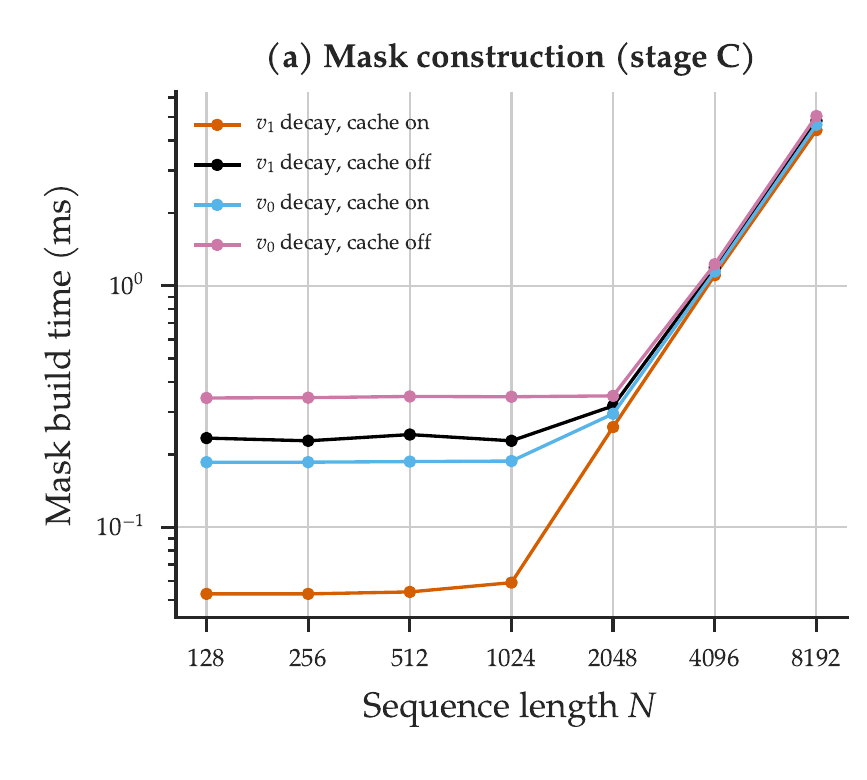
\includegraphics[height=0.56\textheight,keepaspectratio]{mask_construction_panel.png}
    \end{column}
    \begin{column}{0.42\textwidth}
      \centering
      \begin{tikzpicture}[
        card/.style={draw=talkgray!40, fill=talklight, rounded corners=1.5mm,
          text width=38mm, align=center, inner sep=2.2mm, font=\small,
          text=talkgray},
      ]
        \node[card] (one) at (0,0) {%
          {\fontsize{4.5mm}{5.4mm}\selectfont\textcolor{tudblue}{\textbf{4.41 ms}}}\par
          \vspace{1mm}
          {\scriptsize construction at $N{=}8192$}\par
          {\scriptsize 14$\times$ the kernel call}%
        };
        \node[card, below=3mm of one] (two) {%
          {\fontsize{4.5mm}{5.4mm}\selectfont\textcolor{tudblue}{\textbf{1032 MB}}}\par
          \vspace{1mm}
          {\scriptsize bool mask materialization}\par
          {\scriptsize 1.97 ms at $N{=}8192$}%
        };
      \end{tikzpicture}
    \end{column}
  \end{columns}
\end{frame}

% ----------------------------------------------------------------------
% Frame 10 -- cache versus SparseMask.
% (a) Why: the mask can be retained without paying the dense-mask cost.
% (b) Tried: CachedDistAttention distance cache; SparseMask K=16 at B=64.
% (c) Novel: semantics-preserving distance cache; production-batch
%     sparse-mask comparison.
% (d) Interpretation: SparseMask is the practical mask-capable choice;
%     CachedDistAttention is the dense reference. Threat: K=16 only.
% ----------------------------------------------------------------------
\begin{frame}
  \talktitle{If you keep the cutoff, use SparseMask}
  \centering
  \small
  \renewcommand{\arraystretch}{1.35}
  \begin{tabular}{@{}rrrr@{}}
    \toprule
    $N$ & CachedDistAttention (ms) & SparseMask $K{=}16$ (ms) & Speedup\\
    \midrule
    512 & 1.407 & 0.615 & 2.3$\times$\\
    4096 & 85.327 & 21.938 & 3.9$\times$\\
    \bottomrule
  \end{tabular}
  \vspace{5mm}

  {\footnotesize CachedDistAttention caches distances once: 1.26--1.76$\times$ over per-layer recomputation, with identical semantics.\par}
\end{frame}

% ----------------------------------------------------------------------
% Frame 11 -- cutoff ablation.
% (a) Why: the cutoff is often treated as a pure compute knob; test whether
%     removing it is accuracy-neutral.
% (b) Tried: 6-fold leave-one-condition-out, DenseFlash versus
%     CachedDistAttention, 2 seeds.
% (c) Novel: to our knowledge, the first Trackastra cutoff ablation.
% (d) Interpretation: removing the cutoff is not accuracy-neutral; the
%     effect is one-signed but small relative to cross-condition spread.
%     Threat: 2 seeds; no significance test.
% ----------------------------------------------------------------------
\begin{frame}
  \talktitle{Removing the cutoff is not accuracy-neutral}
  \centering
  \small
  \renewcommand{\arraystretch}{1.35}
  \begin{tabular}{@{}p{58mm}p{72mm}@{}}
    \toprule
    \textbf{Result} & \textbf{Value}\\
    \midrule
    Worse fold--seed cells & 12/12 (6 folds $\times$ 2 seeds)\\
    Pooled AOGM penalty & $+47.5$ [32.1, 62.0]\\
    Cutoff occupancy & 42.7\% mean; 23.2\% median\\
    Design & 6-fold leave-one-condition-out; paired\\
    Caveat & 2 seeds; no significance test\\
    \bottomrule
  \end{tabular}
  \vspace{4mm}

  {\footnotesize DenseFlash (cutoff removed) versus CachedDistAttention (cutoff retained).\par}
\end{frame}

% ----------------------------------------------------------------------
% Frame 12 -- equivalence.
% (a) Why: SparseMask can inherit SparseGather's accuracy only if the two
%     implementations agree.
% (b) Tried: 18 configurations, N<=512, K in {4,16}, 3 seeds, fp16.
% (c) Novel: equivalence enabling accuracy transfer without retraining.
% (d) Interpretation: finite numerical agreement, not a proof; valid at the
%     tested configurations. Threat: N<=512.
% ----------------------------------------------------------------------
\begin{frame}
  \talktitle{SparseMask inherits SparseGather accuracy}
  \centering
  \begin{tikzpicture}[
    x=1mm, y=1mm,
    card/.style={draw=talkgray!40, fill=talklight, rounded corners=1.5mm,
      text width=124mm, align=center, inner sep=3mm, minimum height=14mm,
      font=\small, text=talkgray},
  ]
    \node[card, anchor=north] at (72,0)
      {18 configurations; $N{\leq}512$; $K{\in}\{4,16\}$; 3 seeds; fp16};
    \node[card, anchor=north] at (72,-18)
      {Forward $<5\times10^{-4}$; backward $<8\times10^{-4}$};
    \node[card, anchor=north] at (72,-36)
      {$\sim$2 GPU-min versus 600+ for a full training run};
  \end{tikzpicture}
  \vspace{2mm}

  {\footnotesize Finite numerical agreement, not a proof; it licenses accuracy transfer at the tested configurations.\par}
\end{frame}

% ----------------------------------------------------------------------
% Frame 13 -- token reordering.
% (a) Why: the proposal asked whether memory-locality reordering adds gains.
% (b) Tried: SparseGather with spatial token sort on real centroids and
%     random data, L=12, fp16.
% (c) Novel: negative result on real vanvliet centroids.
% (d) Interpretation: negligible gain; discarded. Threat: local measurement.
% ----------------------------------------------------------------------
\begin{frame}
  \talktitle{Token reordering does not help}
  \centering
  \small
  \renewcommand{\arraystretch}{1.35}
  \begin{tabular}{@{}lcc@{}}
    \toprule
    Input & Reorder ratio & Verdict\\
    \midrule
    Real vanvliet centroids\scite{wu2024point} & 0.992--1.023$\times$ & discarded\\
    Random coordinates & 0.97--1.03$\times$ & discarded\\
    \bottomrule
  \end{tabular}
  \vspace{4mm}

  {\footnotesize Proposal item; $L{=}12$; fp16; local measurement.}
\end{frame}

% ----------------------------------------------------------------------
% Frame 14 -- Amdahl and the normalization chain.
% (a) Why: kernel speedup matters only if attention is a large step share.
% (b) Tried: phase decomposition, identity ablation, Amdahl; production loop
%     on five H100 nodes.
% (c) Novel: end-to-end bound with measured shares and the B=1/B=64
%     qualification.
% (d) Interpretation: attention is ~10%; the norm chain is 38.7% and
%     host-side; the measured difference is 2.9% within +/-6%.
%     Threat: per-epoch spread cannot resolve 1.044 vs 1.08.
% ----------------------------------------------------------------------
\begin{frame}
  \talktitle{Attention is not the training bottleneck}
  \centering
  \begin{columns}[c]
    \begin{column}{0.46\textwidth}
      \centering
      {\small\textbf{Step wall}}\par\vspace{1.5mm}
      {\footnotesize
      \renewcommand{\arraystretch}{1.25}
      \begin{tabular}{@{}lr@{}}
        \toprule
        Phase & Share\\
        \midrule
        norm chain & 38.7\%\\
        attention & 10.05\%\\
        other & 51.25\%\\
        \bottomrule
      \end{tabular}}
    \end{column}
    \begin{column}{0.46\textwidth}
      \centering
      {\small\textbf{Amdahl}}\par\vspace{1.5mm}
      {\footnotesize
      \renewcommand{\arraystretch}{1.25}
      \begin{tabular}{@{}lr@{}}
        \toprule
        Assumption & Prediction\\
        \midrule
        $s=0.098$, $k=1.75$ & 1.044\\
        $B{=}64$, $k=6.45$ & $\approx$1.08\\
        measured & 2.9\%, $\pm$6\%\\
        \bottomrule
      \end{tabular}}
    \end{column}
  \end{columns}
  \vspace{3mm}

  {\footnotesize The norm chain is host-side: 240 device synchronizations per step; its GPU kernels are 1.6--2.1\%. Dense baseline (\texttt{knn\_neighbors}$=-1$); the $B{=}1$ $k$ is conservative.\par}
\end{frame}

% ----------------------------------------------------------------------
% Frame 15 -- NSA rejection.
% (a) Why: a sparse-attention candidate was benchmarked and must be resolved.
% (b) Tried: NSA across the measured N grid at B=64.
% (c) Novel: measured rejection at cell-tracking sequence lengths.
% (d) Interpretation: fixed compression and block-selection overhead
%     dominates at small N, not the encoder-decoder architecture.
% ----------------------------------------------------------------------
\begin{frame}
  \talktitle{NSA is rejected at these $N$}
  \centering
  \small
  \renewcommand{\arraystretch}{1.35}
  \begin{tabular}{@{}lr@{}}
    \toprule
    $N$ range & NSA / CachedDistAttention\\
    \midrule
    128--1024 & 11.7$\times$\\
    2048 & 8.5$\times$\\
    4096 & 2.2$\times$\\
    8192 & 1.15$\times$\\
    \bottomrule
  \end{tabular}
  \vspace{4mm}

  {\footnotesize Fixed compression and block-selection overhead dominates at small $N$, not the encoder-decoder architecture.\par}
\end{frame}
